\apendice{Especificación de diseño}

\section{Introducción}

En este apartado se explicarán las especificaciones de diseño utilizadas durante el desarrollo de este proyecto, dividido en varios apartados. Cada uno describe los aspectos clave del sistema y las decisiones tomadas para garantizar su funcionalidad, escalabilidad y eficiencia:

\begin{itemize}
    \item El \textbf{diseño de datos} detalla cómo se organizan, estructuran y gestionan los datos utilizados en el sistema.
    \item El \textbf{diseño procedimental} describe los algoritmos, procesos y flujos operativos implementados en el proyecto.
    \item El \textbf{diseño arquitectónico} define la estructura global del sistema, los componentes principales y las relaciones entre ellos.
\end{itemize}

Los apartados siguientes desglosan cada uno de estos aspectos en detalle.

\section{Diseño de datos}

El diseño de datos de este proyecto se centra en la gestión, almacenamiento y manipulación eficiente de la información utilizada en la aplicación. A continuación, se describen los principales aspectos relacionados con la estructura de los datos, sus fuentes y su tratamiento.

\subsection{Estructura de los datos}

Los datos utilizados en este proyecto consisten en archivos en formato CSV o Excel que representan trayectorias geoespaciales mediante coordenadas GPS. Cada fila del archivo corresponde a una trayectoria individual y contiene atributos esenciales para su análisis. La correcta estructura de los datos es fundamental para garantizar la compatibilidad con el algoritmo TRA-CLUS.

\subsubsection{Requisitos de los datos}

Para que los datos sean procesados correctamente, deben cumplir con los siguientes requisitos:

\begin{itemize}
    \item \textbf{Formato del archivo}: Los datos deben estar almacenados en un archivo delimitado por comas CSV o Excel, compatible con la lectura en Python.
    \item \textbf{Columna \texttt{POLYLINE}}: 
    \begin{itemize}
        \item Es obligatorio que exista una columna llamada \texttt{POLYLINE}.
        \item La columna debe contener las trayectorias GPS en formato JSON, representadas como listas de coordenadas. Ejemplo:
        \[\texttt{[[latitud\_1, longitud\_1], [latitud\_2, longitud\_2], \dots]}\]
    \end{itemize}
    \item \textbf{Ausencia de valores nulos}: No se permiten valores nulos en la columna \texttt{POLYLINE}, ya que esta será la única tratada por el algoritmo.
\end{itemize}

\subsubsection{Motivación del formato}

El formato descrito se adapta específicamente a los requisitos del algoritmo TRA-CLUS. Este diseño asegura que los datos se procesen de manera eficiente, evitando errores y optimizando los cálculos necesarios para identificar patrones en las trayectorias.

\subsection{Modelo de datos}

Para facilitar el procesamiento y análisis de los datos, estos se estructuran internamente en un modelo basado en un \textbf{GeoDataFrame} \cite{geopandas2023}, que permite integrar datos tabulares y geoespaciales de manera eficiente.

\begin{itemize}
    \item Cada fila del \texttt{GeoDataFrame} \cite{geopandas2023} representa una trayectoria única.
    \item Las coordenadas en \texttt{POLYLINE} se convierten en objetos de geometría tipo \texttt{LineString} \cite{shapely2023}, lo que permite su uso en análisis geoespaciales.
\end{itemize}

\subsection{Gestión de datos}

Los datos son procesados en diferentes etapas para asegurar su calidad y consistencia:

\begin{enumerate}
    \item \textbf{Validación:} Se verifica que el archivo cargado cumpla con los requisitos de formato y no contenga valores nulos en columnas clave.
    \item \textbf{Transformación:} Las coordenadas en \texttt{POLYLINE} son transformadas en objetos geoespaciales.
    \item \textbf{Almacenamiento temporal:} Los datos procesados se almacenan temporalmente en memoria para su uso en el análisis y visualización.
    \item \textbf{Exportación:} Los resultados generados (mapas, estadísticas, archivos transformados) se guardan en formato ZIP para su descarga.
\end{enumerate}

\subsection{Almacenamiento de resultados}

Los resultados obtenidos del análisis y ejecución del algoritmo TRACLUS se almacenan en un directorio específico dentro de la aplicación. Este directorio organiza los experimentos realizados en carpetas separadas, garantizando un almacenamiento estructurado y accesible.

Independientemente de los algoritmos seleccionados, siempre se generan los siguientes cuatro archivos comunes:

\begin{itemize}
	\item \textbf{data\_gdf}: contiene todos los datos del archivo CSV o Excel analizado, incluyendo cada trayectoria representada en formato \texttt{LineString}. Este archivo se almacena en formato \texttt{.geojson}.
	\item \textbf{algorithm\_parameters}: archivo \texttt{.txt} que registra los parámetros seleccionados por el usuario para ejecutar el experimento.
	\item \textbf{html\_map}: mapa interactivo en formato HTML que muestra todas las trayectorias sin procesar.
	\item \textbf{html\_heatmap}: mapa de calor en formato HTML basado en los datos sin procesar.
\end{itemize}

Adicionalmente, por cada algoritmo de clustering seleccionado, se generan los siguientes archivos específicos:

\begin{itemize}
	\item \textbf{traclus\_map\_\textit{nombre}}: mapa HTML que representa las trayectorias finales procesadas.
	\item \textbf{traclus\_map\_cluster\_\textit{nombre}}: mapa HTML que visualiza los clusters generados durante el proceso.
	\item \textbf{traclus\_map\_segments\_\textit{nombre}}: mapa HTML que muestra los segmentos obtenidos tras la segmentación.
	\item \textbf{table\_\textit{nombre}}: tabla en formato CSV con las siguientes columnas:
	\begin{itemize}
		\item Número de la trayectoria original.
		\item Segmento al que pertenece.
		\item Cluster asignado.
		\item Trayectoria final resultante.
	\end{itemize}
	\item \textbf{graph\_\textit{nombre}}: tabla en formato CSV que asocia cada segmento con su cluster correspondiente.
\end{itemize}

Los formatos seleccionados priorizan un equilibrio entre velocidad de guardado/cargado y uso eficiente del espacio en memoria. Este diseño asegura que los datos se gestionen de manera eficiente, facilitando tanto la revisión de los experimentos como el análisis y el desarrollo futuro de la aplicación.

\section{Diseño procedimental}

El diseño procedimental de este proyecto define las operaciones clave que realiza la aplicación para cumplir con sus objetivos. Estas operaciones incluyen la carga de datos, el procesamiento de trayectorias, la ejecución del algoritmo TRACLUS, la visualización de resultados y la exportación de datos. A continuación, se detalla el flujo y los procedimientos más importantes.

\begin{figure}[H]
    \centering
    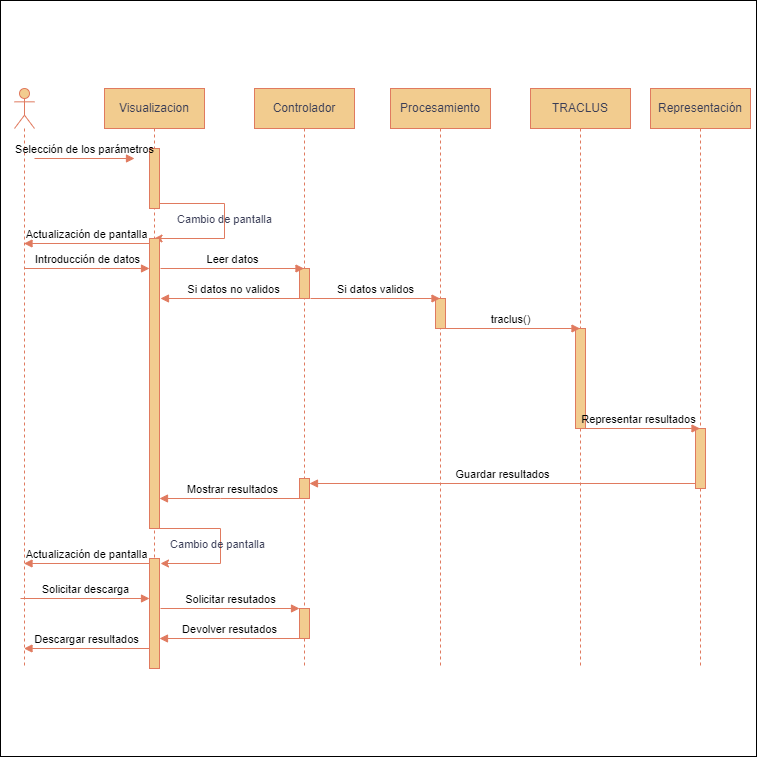
\includegraphics[width=1\textwidth]{img/DiagramaDeSecuencia.png}
    \caption{Diagrama de secuencia.}
\end{figure}

\subsection{Carga y validación de datos}

El proceso comienza con la carga del archivo de datos proporcionado por el usuario. Este procedimiento asegura que los datos estén en el formato correcto antes de continuar.

\begin{enumerate}
    \item El usuario selecciona un archivo CSV o Excel a través de la interfaz.
    \item Se valida el formato del archivo:
    \begin{itemize}
        \item Verificación de la existencia de la columna \texttt{POLYLINE}.
        \item Comprobación de que las coordenadas en \texttt{POLYLINE} estén en un formato JSON válido.
        \item Verificación de que no haya valores nulos en las columnas clave.
    \end{itemize}
    \item Si el archivo es válido, los datos se cargan en memoria como un \texttt{DataFrame} de pandas.
    \item En caso de error, se muestra un mensaje detallado al usuario en la interfaz.
\end{enumerate}

\subsection{Procesamiento de trayectorias}

Una vez cargados los datos, se realiza el procesamiento para convertir las trayectorias en un formato adecuado para el análisis.

\begin{itemize}
    \item Las coordenadas GPS en la columna \texttt{POLYLINE} se transforman en objetos \texttt{LineString} utilizando la biblioteca \texttt{shapely}.
    \item Se crea un \texttt{GeoDataFrame} que combina datos tabulares con las trayectorias geoespaciales.
    \item Este \texttt{GeoDataFrame} se almacena temporalmente en memoria para los siguientes pasos.
\end{itemize}

\subsection{Ejecución del algoritmo TRACLUS}

El algoritmo TRACLUS se utiliza para agrupar trayectorias similares en clústeres.

\begin{enumerate}
    \item Los parámetros del algoritmo son definidos por el usuario, dependiendo del método de clustering seleccionado:
    \begin{itemize}
        \item Número mínimo de puntos por clúster (\texttt{SpectralClustering}).
        \item Distancia máxima entre segmentos (\texttt{OPTICS}).
    \end{itemize}
    \item Se realiza un preprocesamiento para dividir las trayectorias en segmentos.
    \item El algoritmo TRACLUS agrupa los segmentos en clústeres basados en su proximidad y similitud.
    \item Los resultados incluyen:
    \begin{itemize}
        \item Trayectorias agrupadas por clúster.
        \item Trayectorias representativas de cada clúster.
    \end{itemize}
\end{enumerate}

\subsection{Visualización de resultados}

Los resultados del algoritmo se representan visualmente en mapas interactivos. Todos estos datos se almacenan dentro de la aplicación para poder acceder a ellos en el futuro, y los datos actualmente utilizados se guardan en variables globales para reducir los tiempos de carga entre las pantallas de visualización.

\begin{itemize}
    \item La página inicial muestra las trayectorias originales en un mapa.
    \item Los resultados del clustering se visualizan en una página específica, donde cada clúster se representa con un color diferente.
    \item Se incluyen gráficos estadísticos que resumen la distribución de los clústeres.
\end{itemize}

\subsection{Exportación de resultados}

El sistema permite al usuario descargar los resultados del análisis en un archivo ZIP.

\begin{itemize}
    \item El archivo ZIP incluye:
    \begin{itemize}
        \item Mapas en formato PNG.
        \item Archivos CSV con los datos procesados y los clústeres generados.
    \end{itemize}
\end{itemize}

\subsection{Conclusión}

El diseño procedimental asegura un flujo lógico y eficiente desde la carga de datos hasta la exportación de resultados. Cada paso está diseñado para ser modular y reutilizable, lo que facilita la adaptación del sistema a futuros cambios o mejoras.

\section{Diseño arquitectónico}

El diseño arquitectónico de este proyecto sigue el modelo \textbf{Vista-Controlador (MVC)}. Este patrón organiza la aplicación en tres componentes principales: el modelo, la vista y el controlador. Adicionalmente, se ha incluido un componente complementario denominado \textbf{Utils} para funciones auxiliares, lo que asegura una separación clara de responsabilidades, facilita el mantenimiento y mejora la escalabilidad del sistema.

\subsection{Estructura general del modelo MVC}

\begin{itemize}
    \item \textbf{Modelo (Model):}
    \begin{itemize}
        \item Responsable de la gestión de los datos y la lógica de negocio.
        \item Incluye funciones para la validación, procesamiento y almacenamiento temporal de datos.
        \item Implementado mediante estructuras como \texttt{DataFrame} y \texttt{GeoDataFrame}.
    \end{itemize}
    \item \textbf{Vista (View):}
    \begin{itemize}
        \item Encargada de la interacción con el usuario mediante una interfaz gráfica.
        \item Desarrollada utilizando \textbf{Dash}, que aprovecha componentes de React para crear layouts interactivos.
        \item Proporciona pantallas para la carga de datos, la selección de parámetros y la visualización de resultados.
    \end{itemize}
    \item \textbf{Controlador (Controller):}
    \begin{itemize}
        \item Actúa como intermediario entre el modelo y la vista.
        \item Gestiona las peticiones del usuario, realiza las operaciones necesarias en el modelo y actualiza la vista con los resultados.
        \item Incluye la lógica de los \texttt{callbacks} de Dash y otras funciones de control específicas.
    \end{itemize}
    \item \textbf{Funciones complementarias (Utils):}
    \begin{itemize}
        \item Proveen soporte adicional para transformar y gestionar datos utilizados por la vista y el controlador.
        \item Contienen variables globales para almacenar información compartida.
        \item Ayudan en tareas como guardar y cargar datos, reduciendo la complejidad del controlador.
    \end{itemize}
\end{itemize}

\subsection{Diagrama de arquitectura MVC}

El siguiente diagrama ilustra cómo se organizan e interactúan los componentes del modelo MVC en este proyecto:

\begin{figure}[H]
    \centering
    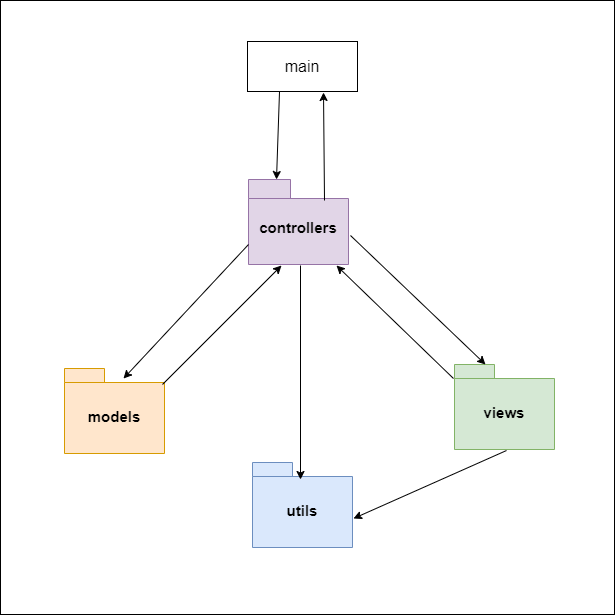
\includegraphics[width=0.9\textwidth]{img/vistacontrolador.png}
    \caption{Diagrama de clases, carpetas.}
\end{figure}


\subsection{Flujo de operaciones}

El flujo de operaciones en la arquitectura MVC sigue estos pasos principales:

\begin{enumerate}
    \item El usuario interactúa con la \textbf{vista} (por ejemplo, carga un archivo, selecciona parámetros o solicita un análisis).
    \item La \textbf{vista} envía los eventos generados al \textbf{controlador}.
    \item El \textbf{controlador} procesa las solicitudes y realiza las operaciones necesarias en el \textbf{modelo}.
    \item El \textbf{modelo} devuelve los resultados al \textbf{controlador}.
    \item El \textbf{controlador} actualiza la \textbf{vista} con los resultados para que el usuario pueda visualizarlos.
\end{enumerate}

\subsection{Organización del código}

El proyecto está organizado para reflejar la arquitectura MVC, con las siguientes carpetas principales:

\begin{itemize}
    \item \textbf{Main:} Contiene el archivo principal que ejecuta el programa (\texttt{main.py}).
    \item \textbf{Modelo (Model):} Almacenado en la carpeta \texttt{models}, incluye funciones para el procesamiento de trayectorias, validación de datos y almacenamiento temporal.
    
\begin{figure}[H]
    \centering
    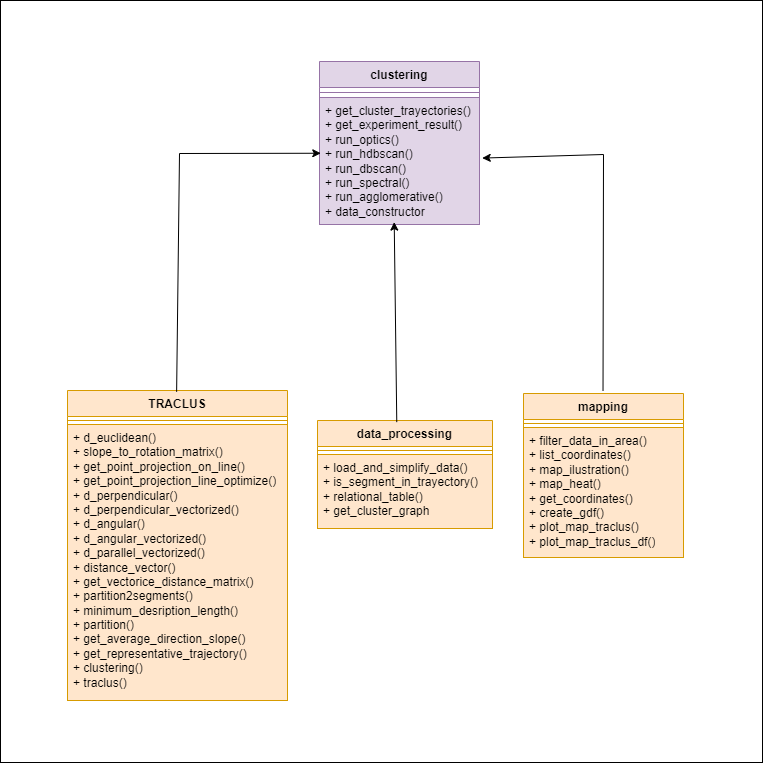
\includegraphics[width=0.9\textwidth]{img/Models.png}
    \caption{Diagrama de clases, relaciones modelos.}
\end{figure}
    
    
    \item \textbf{Vista (View):} Situado en la carpeta \texttt{views}, contiene los layouts y componentes visuales de Dash.
    
\begin{figure}[H]
    \centering
    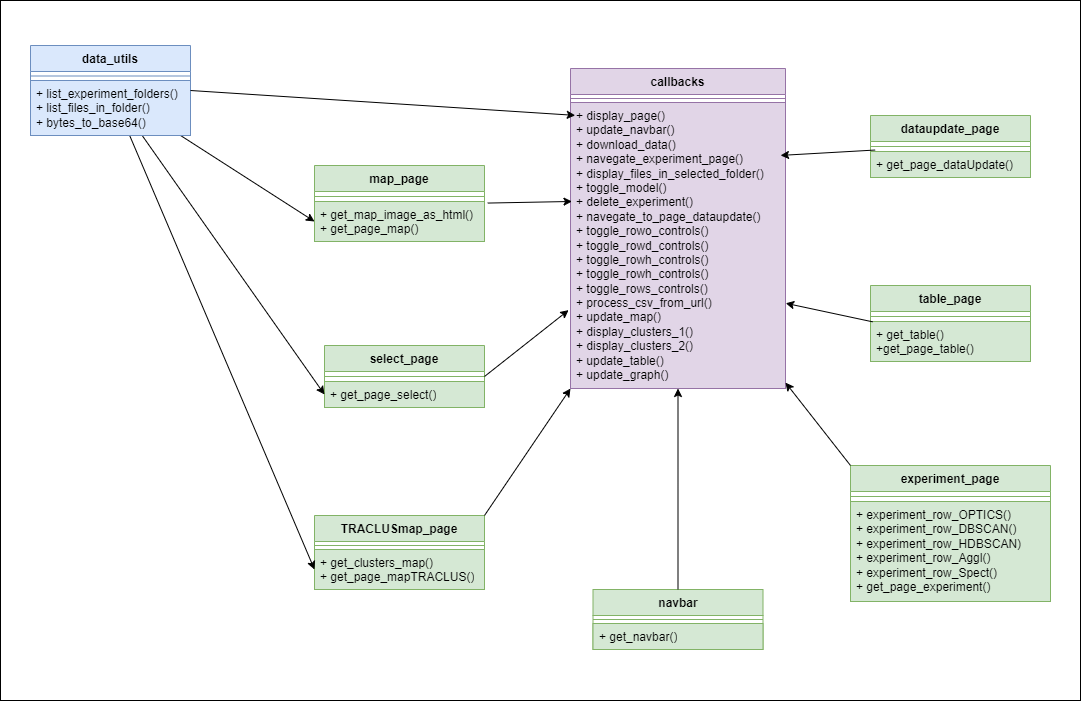
\includegraphics[width=0.9\textwidth]{img/Views.png}
    \caption{Diagrama de clases, relaciones vistas.}
\end{figure}


    \item \textbf{Controlador (Controller):} Ubicado en la carpeta \texttt{controllers}, implementa la lógica de los \texttt{callbacks} de Dash y coordina las operaciones entre el modelo y la vista.
    
\begin{figure}[H]
    \centering
    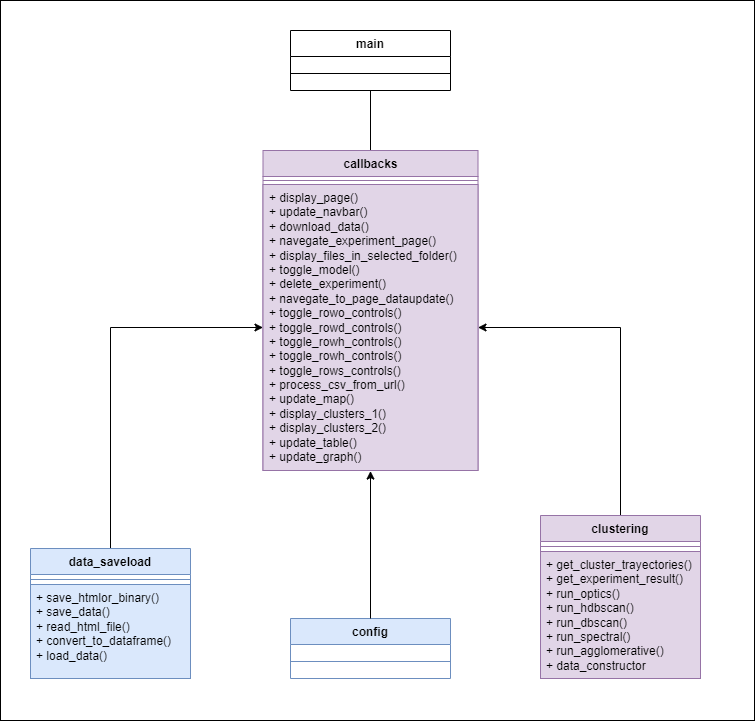
\includegraphics[width=0.9\textwidth]{img/Controllers.png}
    \caption{Diagrama de clases, relaciones controladores.}
\end{figure}


    \item \textbf{Funciones complementarias (Utils):} Localizado en la carpeta \texttt{utils}, proporciona herramientas auxiliares y funciones adicionales para el controlador y la vista.
\end{itemize}

\subsection{Conclusión}

La implementación del modelo MVC en este proyecto asegura una separación clara de responsabilidades entre los componentes, permitiendo que cada uno se desarrolle, pruebe y modifique de manera independiente. Esta arquitectura no solo mejora la mantenibilidad del sistema, sino que también facilita su escalabilidad, permitiendo agregar nuevas funcionalidades sin comprometer la estabilidad general del proyecto.
